\chapter[Valutazione]{Valutazione delle prestazioni del sistema in condizioni di uso reali.}

\begin{figure}
	\centering
		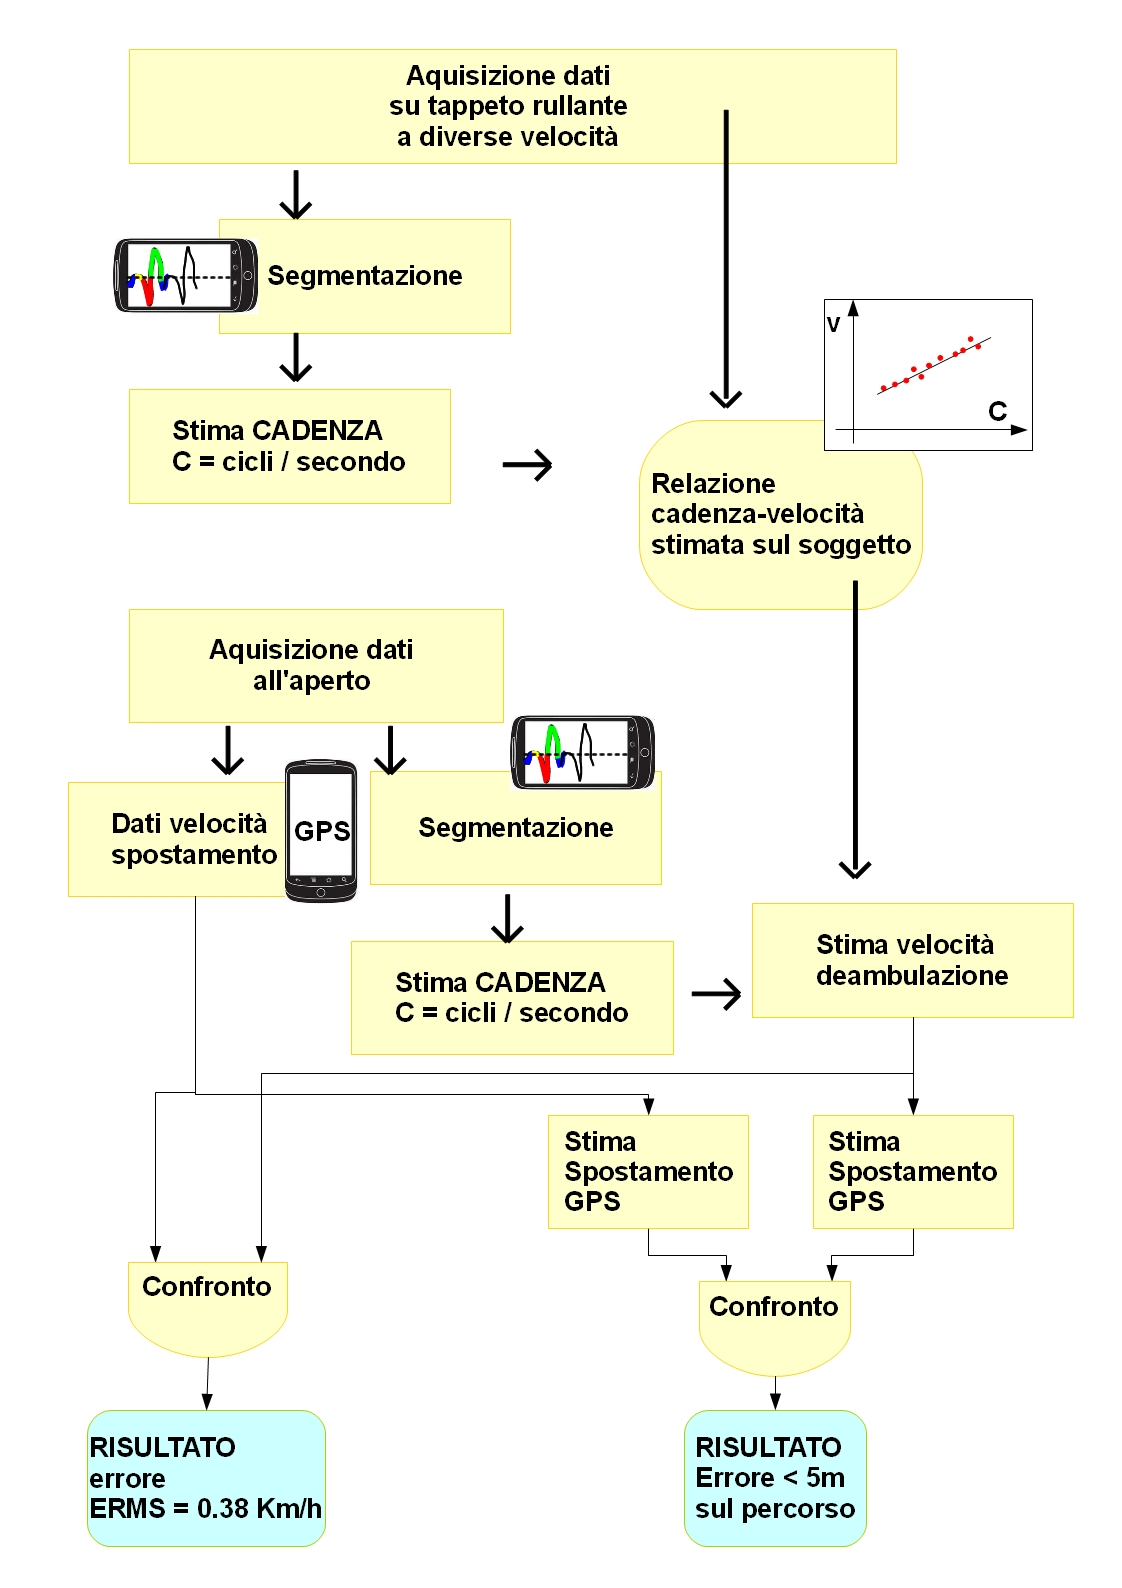
\includegraphics[width=1\textwidth]{imgs/ValutazionePrestazioniSistema.jpg}
	\caption{Segnale di un giroscopio posizionato sul piede.}
	\label{fig:gyroPattern}
\end{figure}

Per valutare le prestazioni del modello in condizioni di uso reale � stato pensato un sistema a due fasi (vedi figura \ref{fig:gyroPattern}): 

\begin{enumerate}
	\item Fase di lavoro in laboratorio 
	
		\begin{description}
		\item [Acquisizione Dati in laboratorio] sono stati acquisiti dati di deambulazione (vedi tabella 	 \ref{tab:TabellaRiassuntivaRaccoltaDatiLab}).
	Le prove sono state compiute su un tappeto rullante con pendenza 0�, nell'intervallo di velocit� [2-8]Km/h. La prima sessione alla velocit� di 2Km/h e con un incremento di 1Km/h in ciascuna sessione successiva. Ciascuna sessione � stata della durata di 1:30 minuti.
	\begin{table}[htbp]
		\centering
		\begin{tabular}{|l|c|}
			\hline		
				\textbf{Attivit�}& cammino\\
				\hline
				\textbf{Soggetti}& 1\\
				\hline
				\textbf{Velocit�}& \{2,3,4,5,6,7,8\}Km/h\\
				\hline
				\textbf{Durata}& \multicolumn{1}{c|}{1:30 minuti per attivit�}\\
				\hline
				\textbf{Strumenti} & \multicolumn{1}{c|}{IMU, Smartphone, tappeto rullante}\\
				\hline
				\textbf{Luogo}& \multicolumn{1}{c|}{Laboratorio}\\
				\hline
				\textbf{Dati raccolti} & \multicolumn{1}{c|}{valori giroscopio segmentati}\\
				\hline
				\textbf{Frequenza campionamento} & \multicolumn{1}{c|}{100 Hz}\\
				\hline
			\end{tabular}
		\caption{Riassunto della raccolti dati in laboratorio}
		\label{tab:TabellaRiassuntivaRaccoltaDatiLab}
	\end{table}
	
	Le sessioni sono state tutte eseguite posizionando saldamente una IMU (vedi appendice \ref{sec:sensori}) sul collo del piede dei soggetti mediante un cinturino in velcro. Il tipo di sensore usato � un giroscopio monoassiale con asse di sensibilit� orientato sul piano mediale-laterale (sagittale) (vedi figura \ref{fig:HumanBodySPL}).\\ 
	I dati sono stati raccolti mediante l'applicazione implementata su \textit{Smartphone}, con relativa segmentazione. 
	
	\item [Stima della cadenza] $c_{LAB}$, la cadenza come definita in tabella \ref{parametri_velocit�} � il numero di cicli di deambulazione per unit� di tempo (cicli/secondo). Dalla segmentazione si hanno implicitamente i passi, in quanto � sufficiente contare il numero di volte che si presenta un dato evento (ad esempio HS) in un unit� di tempo. \TODO{mettere il valore della cadenza ottenuta}.
	\item [Relazione fra cadenza e velocit� stimata sul soggetto] dato che le prove sono state fatte su un tappeto rullante, la velocit� � sempre nota (vedi tabella \ref{tab:TabellaRiassuntivaRaccoltaDatiLab}). L'obbiettivo � trovare una relazione tra la cadenza calcolata e la velocit� nota, mediante una regressione.
	\begin{table}[htbp]
		\centering
		\begin{tabular}{|l|c|}
			\hline		
				\textbf{velocit� in Km}& \textbf{cadenza - cicli/s}\\
				\hline
				2&?\\			
				\hline
				3&?\\			
				\hline
				4&?\\			
				\hline
				5&?\\			
				\hline
				6&?\\			
				\hline
				7&?\\			
				\hline
				8&?\\			
				\hline
		\end{tabular}
		\caption{Cadenza calcolata per ogni velocit� del tappeto rullante.}
		\label{tab:relazioneCadenzaVelocit�}
	\end{table}
	\end{description}
	
		\item Fase di lavoro all'aria aperta
	\begin{description}
		\item [Acquisizione dati giroscopio e segmentazione] all'aria aperta sono stati acquisiti dati di deambulazione (vedi tabella \ref{tab:TabellaRiassuntivaRaccoltaDatiAperto}). Le prove sono state compiute su un percorso piano (pendenza media 0�), ad andatura a velocit� normale per il soggetto in questione. La sessione � stata della durata di \TODO{10 minuti}.
		\begin{table}[htbp]
		\centering
		\begin{tabular}{|l|c|}
			\hline		
				\textbf{Attivit�}& cammino\\
				\hline
				\textbf{Soggetti}& 1\\
				\hline
				\textbf{Velocit�}& $\approx 5 Km/h$\\
				\hline
				\textbf{Durata}& \multicolumn{1}{c|}{10 minuti }\\
				\hline
				\textbf{Strumenti} & \multicolumn{1}{c|}{IMU, Smartphone}\\
				\hline
				\textbf{Luogo}& \multicolumn{1}{c|}{Aperto}\\
				\hline
				\textbf{Dati raccolti} & \multicolumn{1}{c|}{valori giroscopio segmentati}\\
				\hline
				\textbf{Frequenza campionamento} & \multicolumn{1}{c|}{100 Hz}\\
				\hline
			\end{tabular}
		\caption{Riassunto della procedura di raccolta dei dati all'aperto.}
		\label{tab:TabellaRiassuntivaRaccoltaDatiAperto}
	\end{table}
	\item [Stima della cadenza] $c_{OUT}$, la cadenza � stata calcolata con la stessa procedura della fase precedente.
	
	\item [Stima della velocit� di deambulazione] $IMUspeed$,  a partire dalla relazione tra cadenza e velocit� ottenuta nella fase precedente (vedi tabella \ref{tab:relazioneCadenzaVelocit�}) e dalla cadenza stimata nella seconda fase del lavoro, � stata fatta una stima della velocit� di deambulazione all'aperto. 
	
	\item [Stima della distanza percorsa] $IMUdistance$, dato che il tempo di percorrenza � noto, dalla stima di velocit� si ottiene anche la distanza percorsa.
	\begin{equation}
\begin{split}
\displaystyle IMUdistance = \int_{t_{start}}^{t_{end}}{IMUspeed} \; dt\\
\end{split}
\label{eq:IMUdistance}
\end{equation}

	\item [Acquisizione dati GPS] contemporaneamente alla segmentazione, mediante il dispositivo GPS \footnote{Global Positioning System} integrato nello \textit{Smartphone}, sono state acquisite la velocit� di spostamento $GPSspeed$ e la distanza percorsa. I dati acquisiti sulla distanza percorsa sono stai scartati in quanto con margine di errore elevato. 

		\item [Stima della distanza percorsa mediante GPS] $GPSdistance$, dato che il tempo di percorrenza � noto, dai dati di velocit� acquisiti mediante il GPS si ottiene la distanza percorsa. 
				
\begin{equation}
\begin{split}
\displaystyle GPSdistance = \int_{t_{start}}^{t_{end}}{GPSspeed} \; dt\\
\end{split}
\label{eq:GPSdistance}
\end{equation}

	\item [Confronto velocit�]: le due velocit� vengono comparate (vedi figura \ref{fig:IMUspeedGPSspeedVStime}, \ref{fig:IMUspeedVSGPSspeed}, \ref{fig:IMUspeedVSGPSspeedBA}). Lo scarto quadratico medio (\textit{Root Mean Square}) al termine del tempo di acquisizione � 
	\begin{equation}
	1/2 * (\sqrt{IMUspeed^2 + GPSspeed^2}) = 0.38Km/h
	\label{eq:ermsSpeed}
	\end{equation}
	\item [Confronto distanza]: le due distanze vengono confrontate (vedi figura \ref{fig:IMUdistanceGPSdistanceVStime}, \ref{fig:IMUdistanceVSGPSdistance}, ). Misurando la differenza fra le distanze calcolate, si vede che a termine del periodo di acquisizione dei dati (circa 2 minuti) vi � una deriva della $IMUdistance$ di $5m$.
	\begin{equation}
	|IMUdistance - GPSdistance| < 5m
	\label{eq:ermsDistance}
	\end{equation}
	
	\end{description}
\end{enumerate} 
